\chapter{Molecular mechanisms of aspartate limitation}
blaa

\section{Introduction}
More blaa

\subsection{Intro subject 1}
qwerty

\subsection{Intro subject 2}
qwerty
\subsection{Details}
qwerty1




\section{Quantifying the metabolic fates of aspartate}



\begin{figure}
     \centering
     \begin{subfigure}[b]{0.7\textwidth}
         \centering
         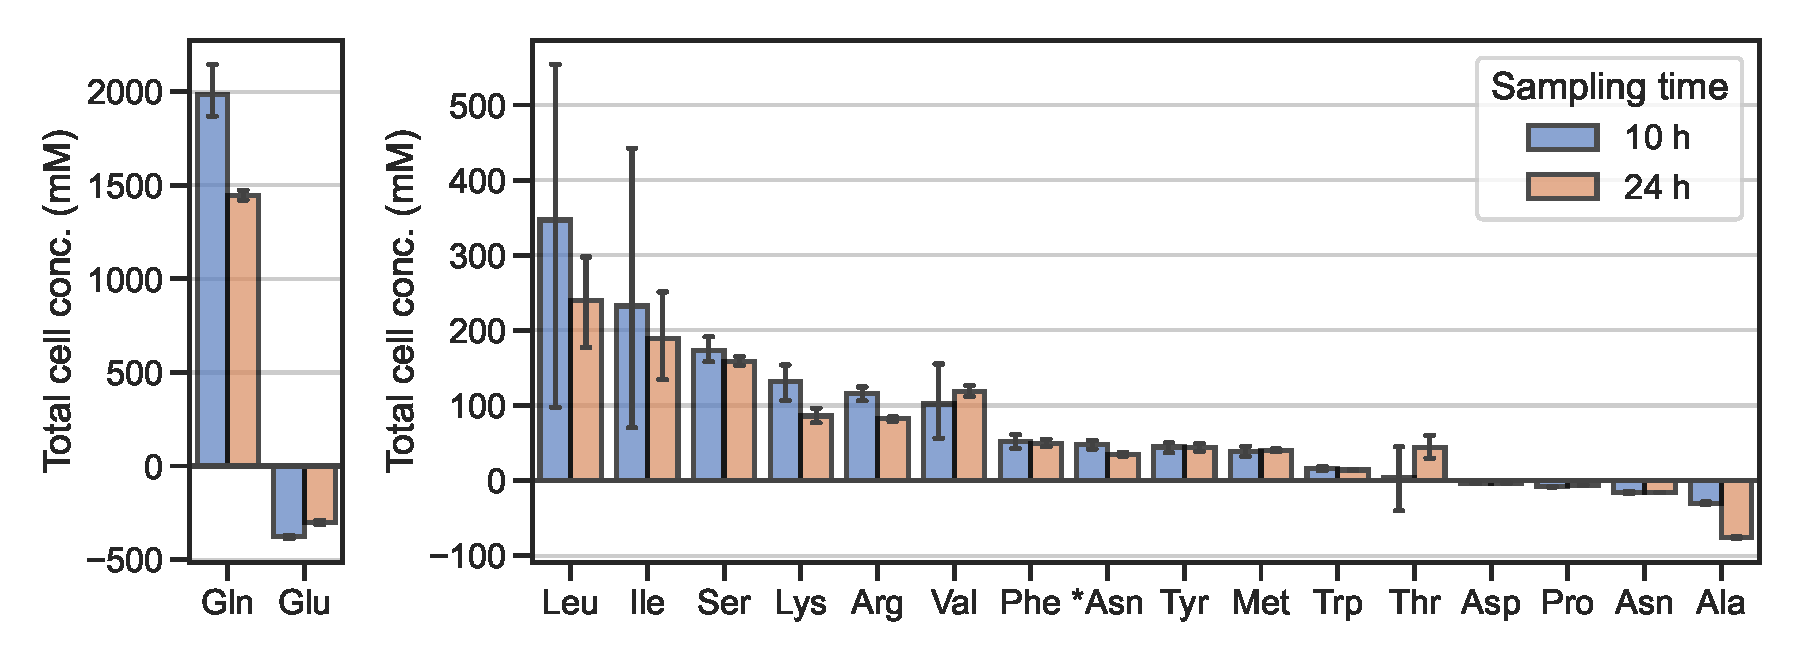
\includegraphics[width=\textwidth]{figures/chap2/tcc_143wt.pdf}
         \caption{Media uptake 143B WT}
         \label{fig:tcc_143wt}
     \end{subfigure}
     %\hfill
     \begin{subfigure}[b]{0.7\textwidth}
         \centering
         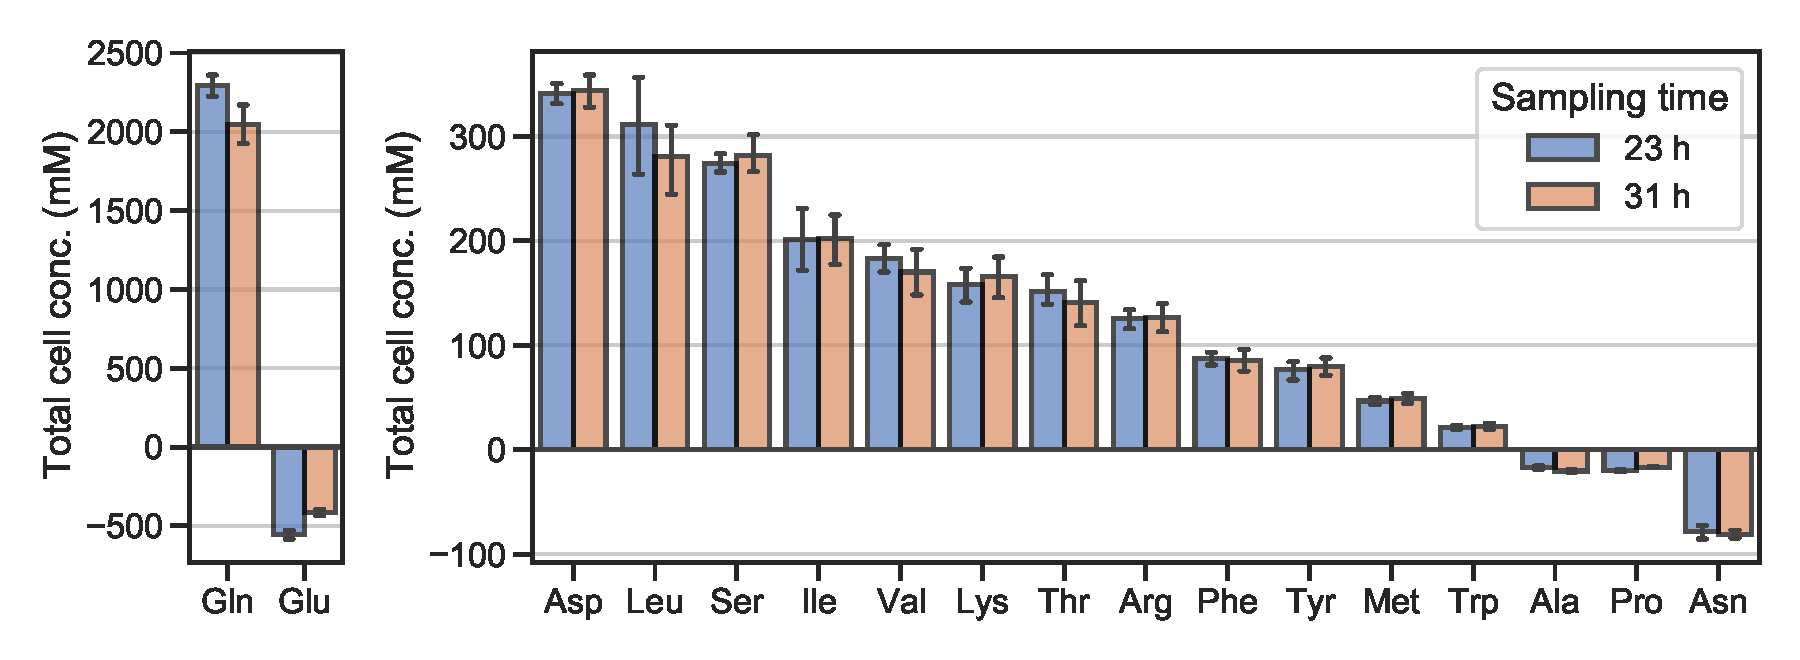
\includegraphics[width=\textwidth]{figures/chap2/tcc_143dko.pdf}
         \caption{Media uptake 143B GOT DKO}
         \label{fig:tcc_143dko}
     \end{subfigure}
        \caption[fff]{
        (a) hhhh, (b) gggg.
        }
\end{figure}













\section{Salvage of the metabolic fates of aspartate}

\subsection{Salvage mix fulfills all the metabolic fates of aspartate}

metabolic fates of aspartate i.e. aspartate conversion 


\begin{figure}
    \centering
    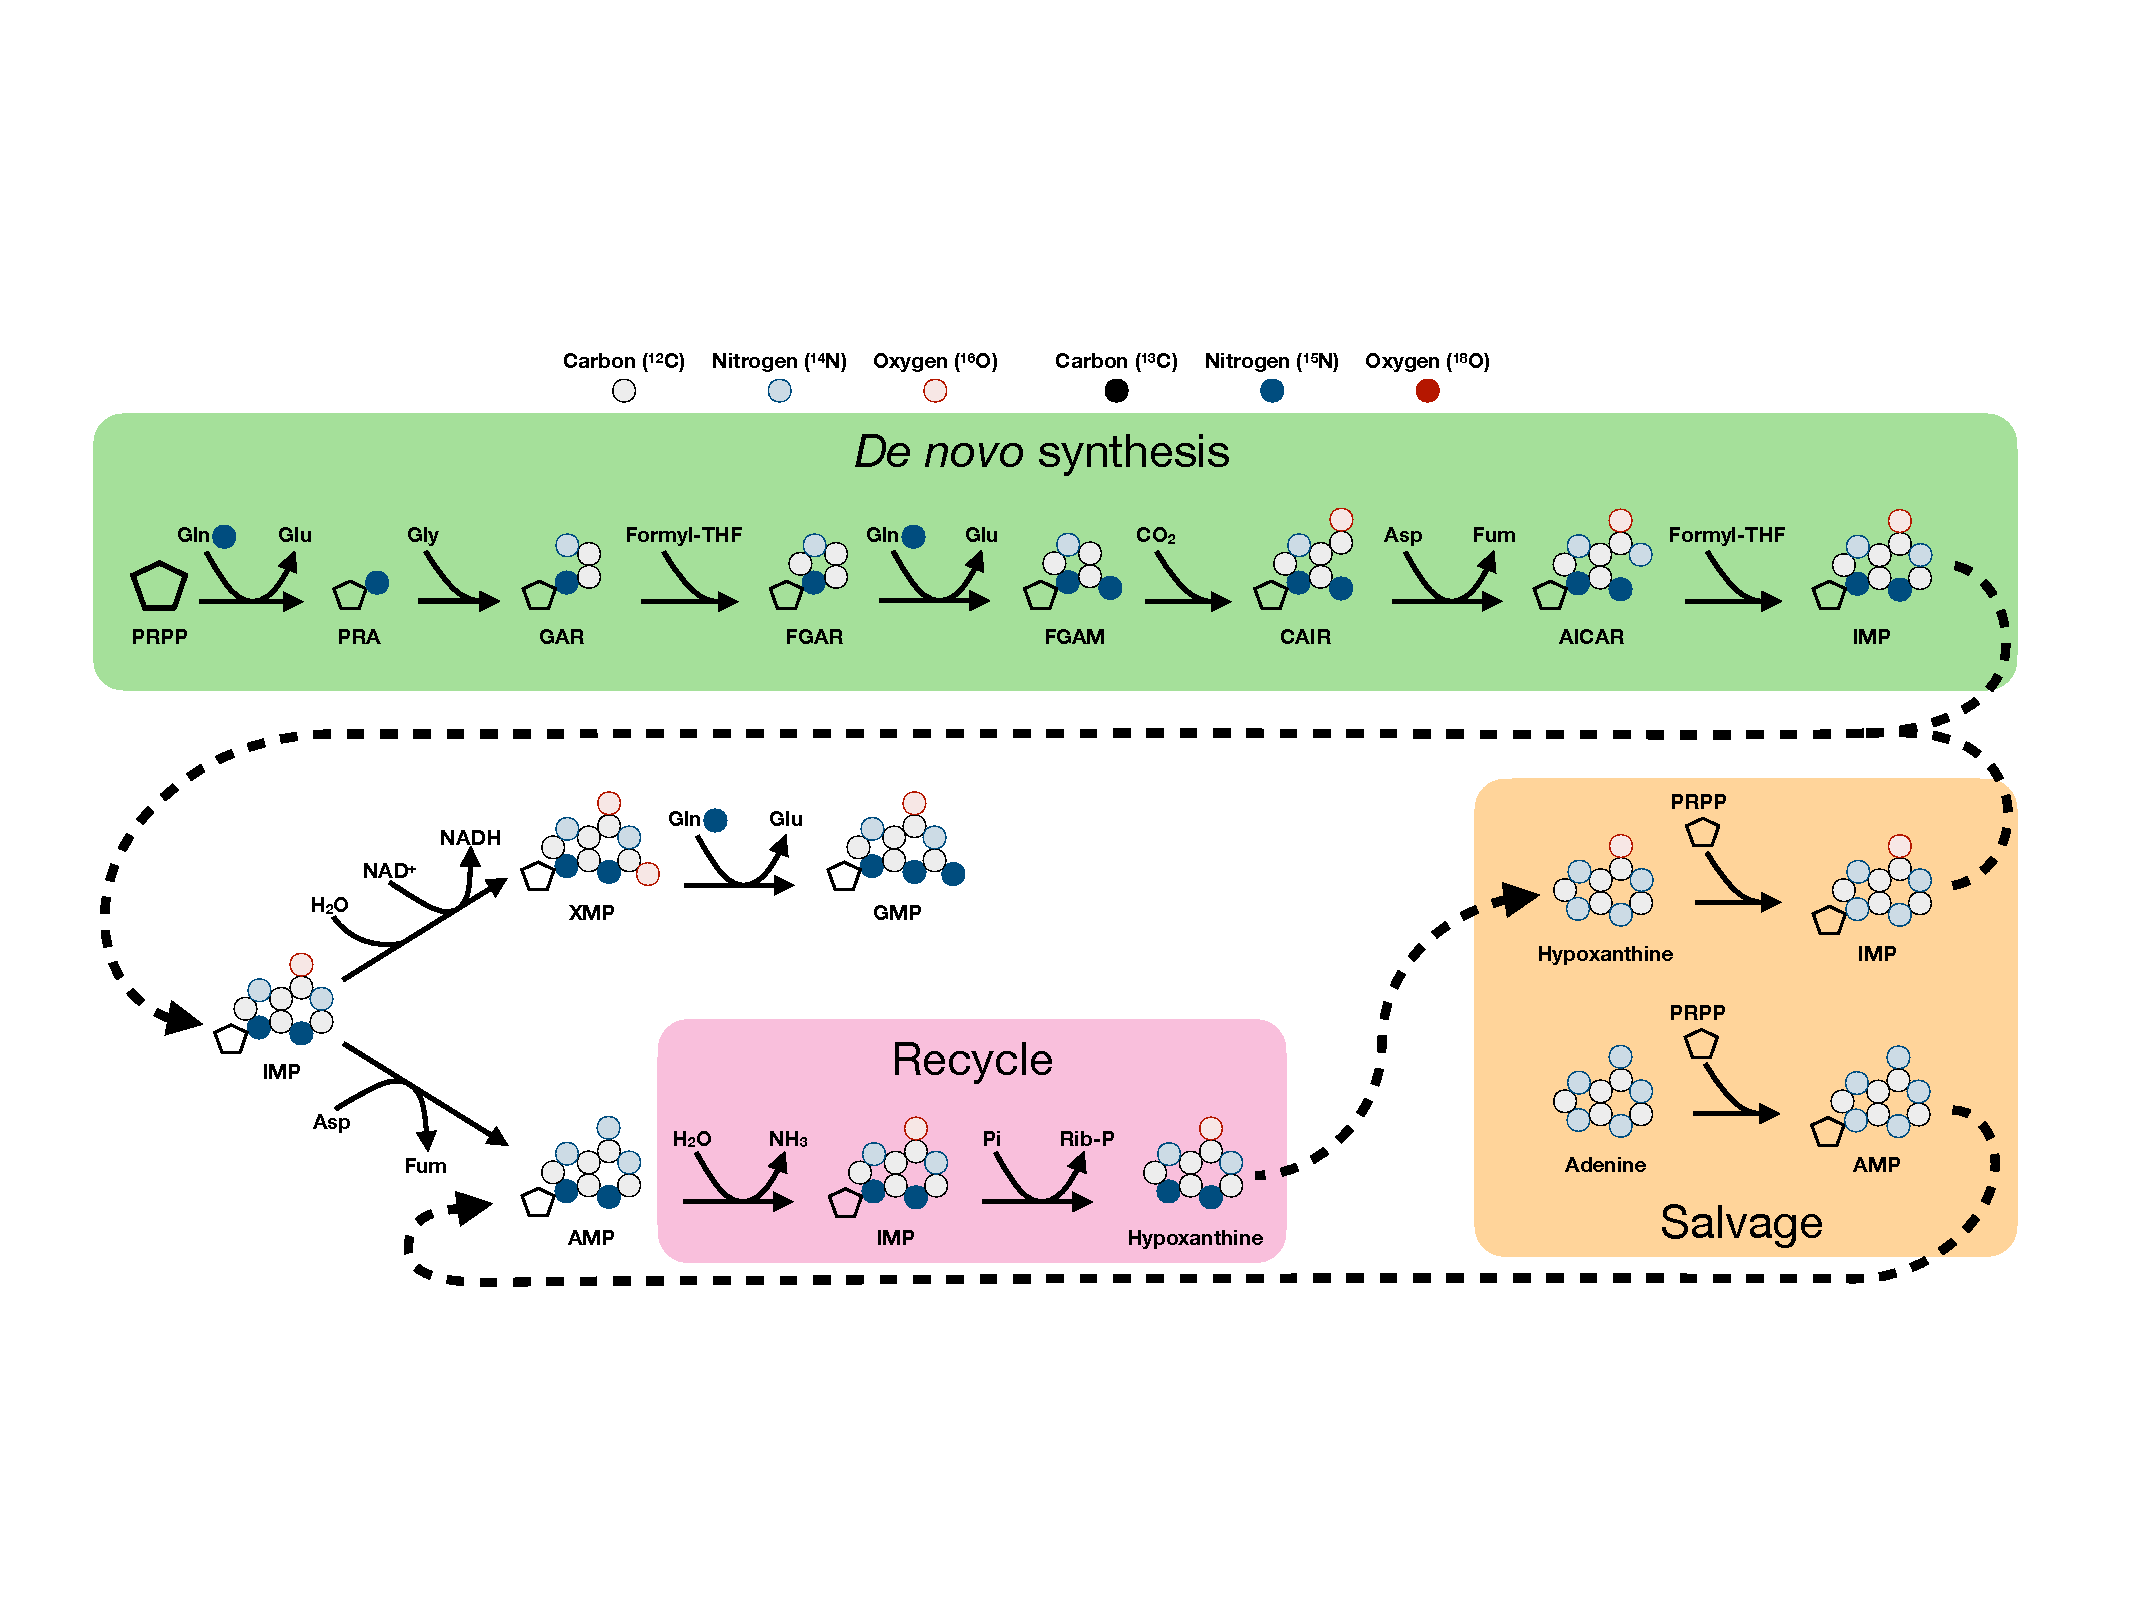
\includegraphics[width=0.95\textwidth]{figures/chap2/purine_tracing_overvew.pdf}
    \caption[Purine metabolism \textsuperscript{15}N-amide Gln tracing overview]{
    Overview of \textsuperscript{15}N-amide Gln label incorporation in \textit{de novo} purine synthesis.
    Label incorporation can be effected by salvage of unlabelled hypoxanthine or adenine and recycling as it appears on the overview.
    }
    \label{fig:ch2:pur_tr_ov}
\end{figure}





\begin{figure}
    \centering
    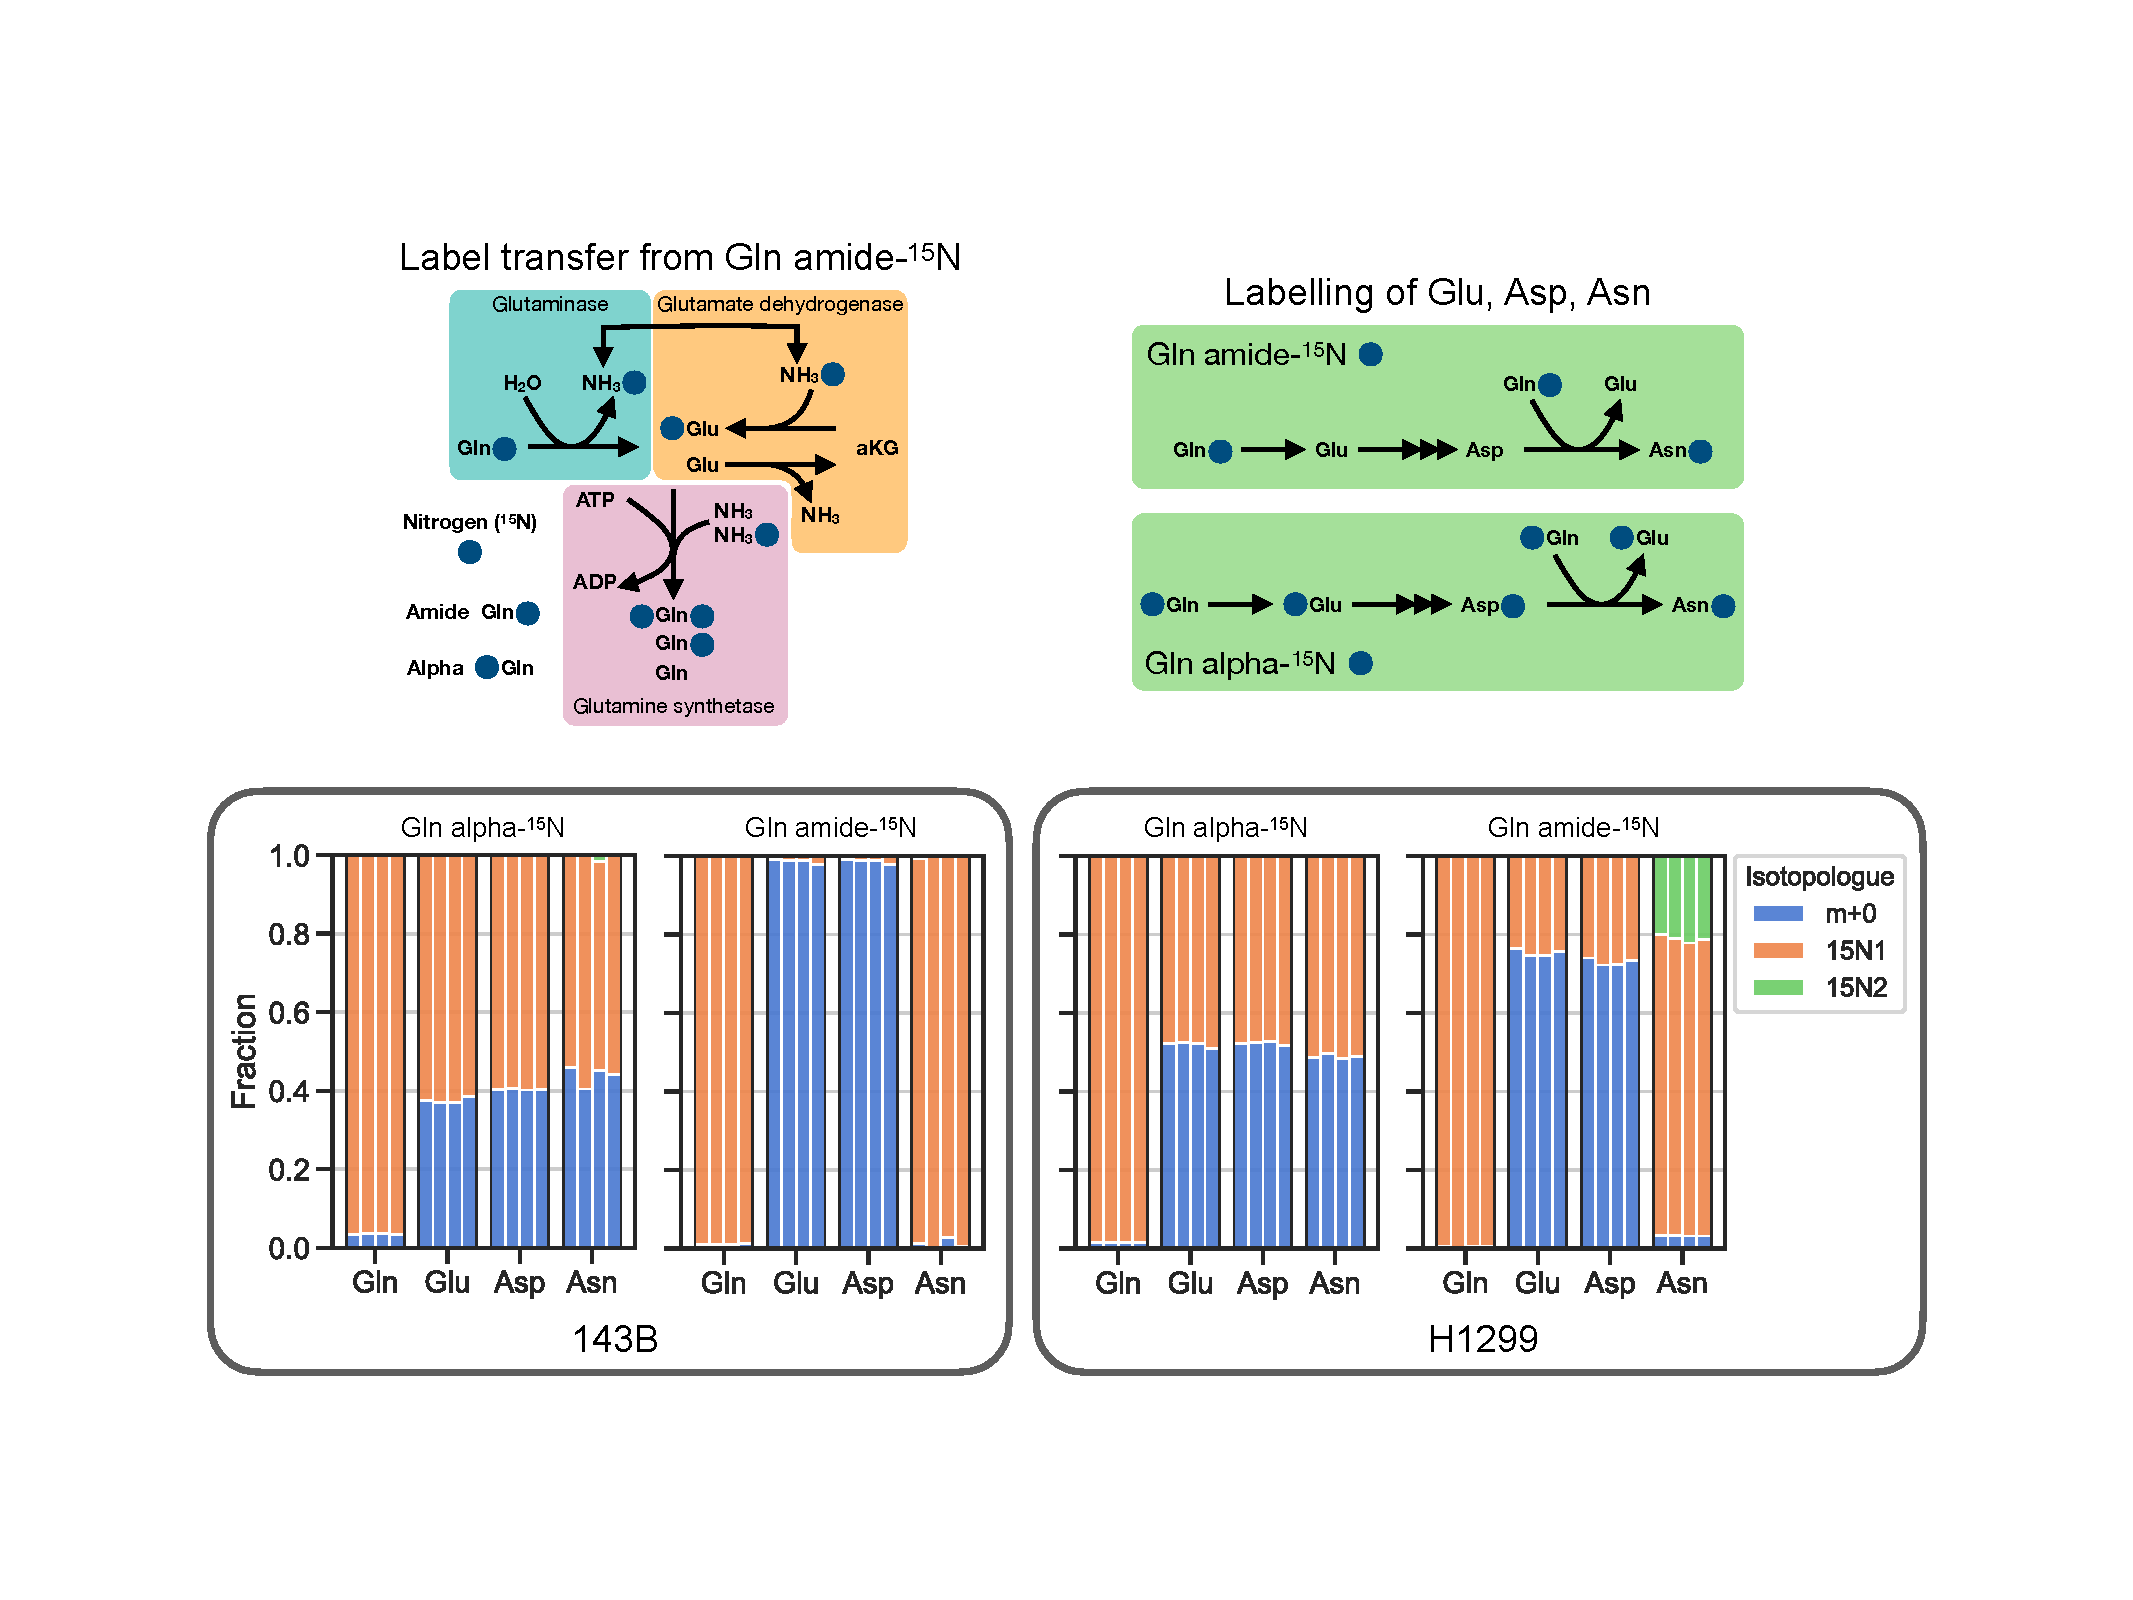
\includegraphics[width=0.95\textwidth]{figures/chap2/gln_lab_tranfr.pdf}
    \caption[Gln amide to alpha \textsuperscript{15}N transfer]{
    ggg
    }
    \label{fig:ch2:gln_lab_tranfr}
\end{figure}


\begin{figure}
    \centering
    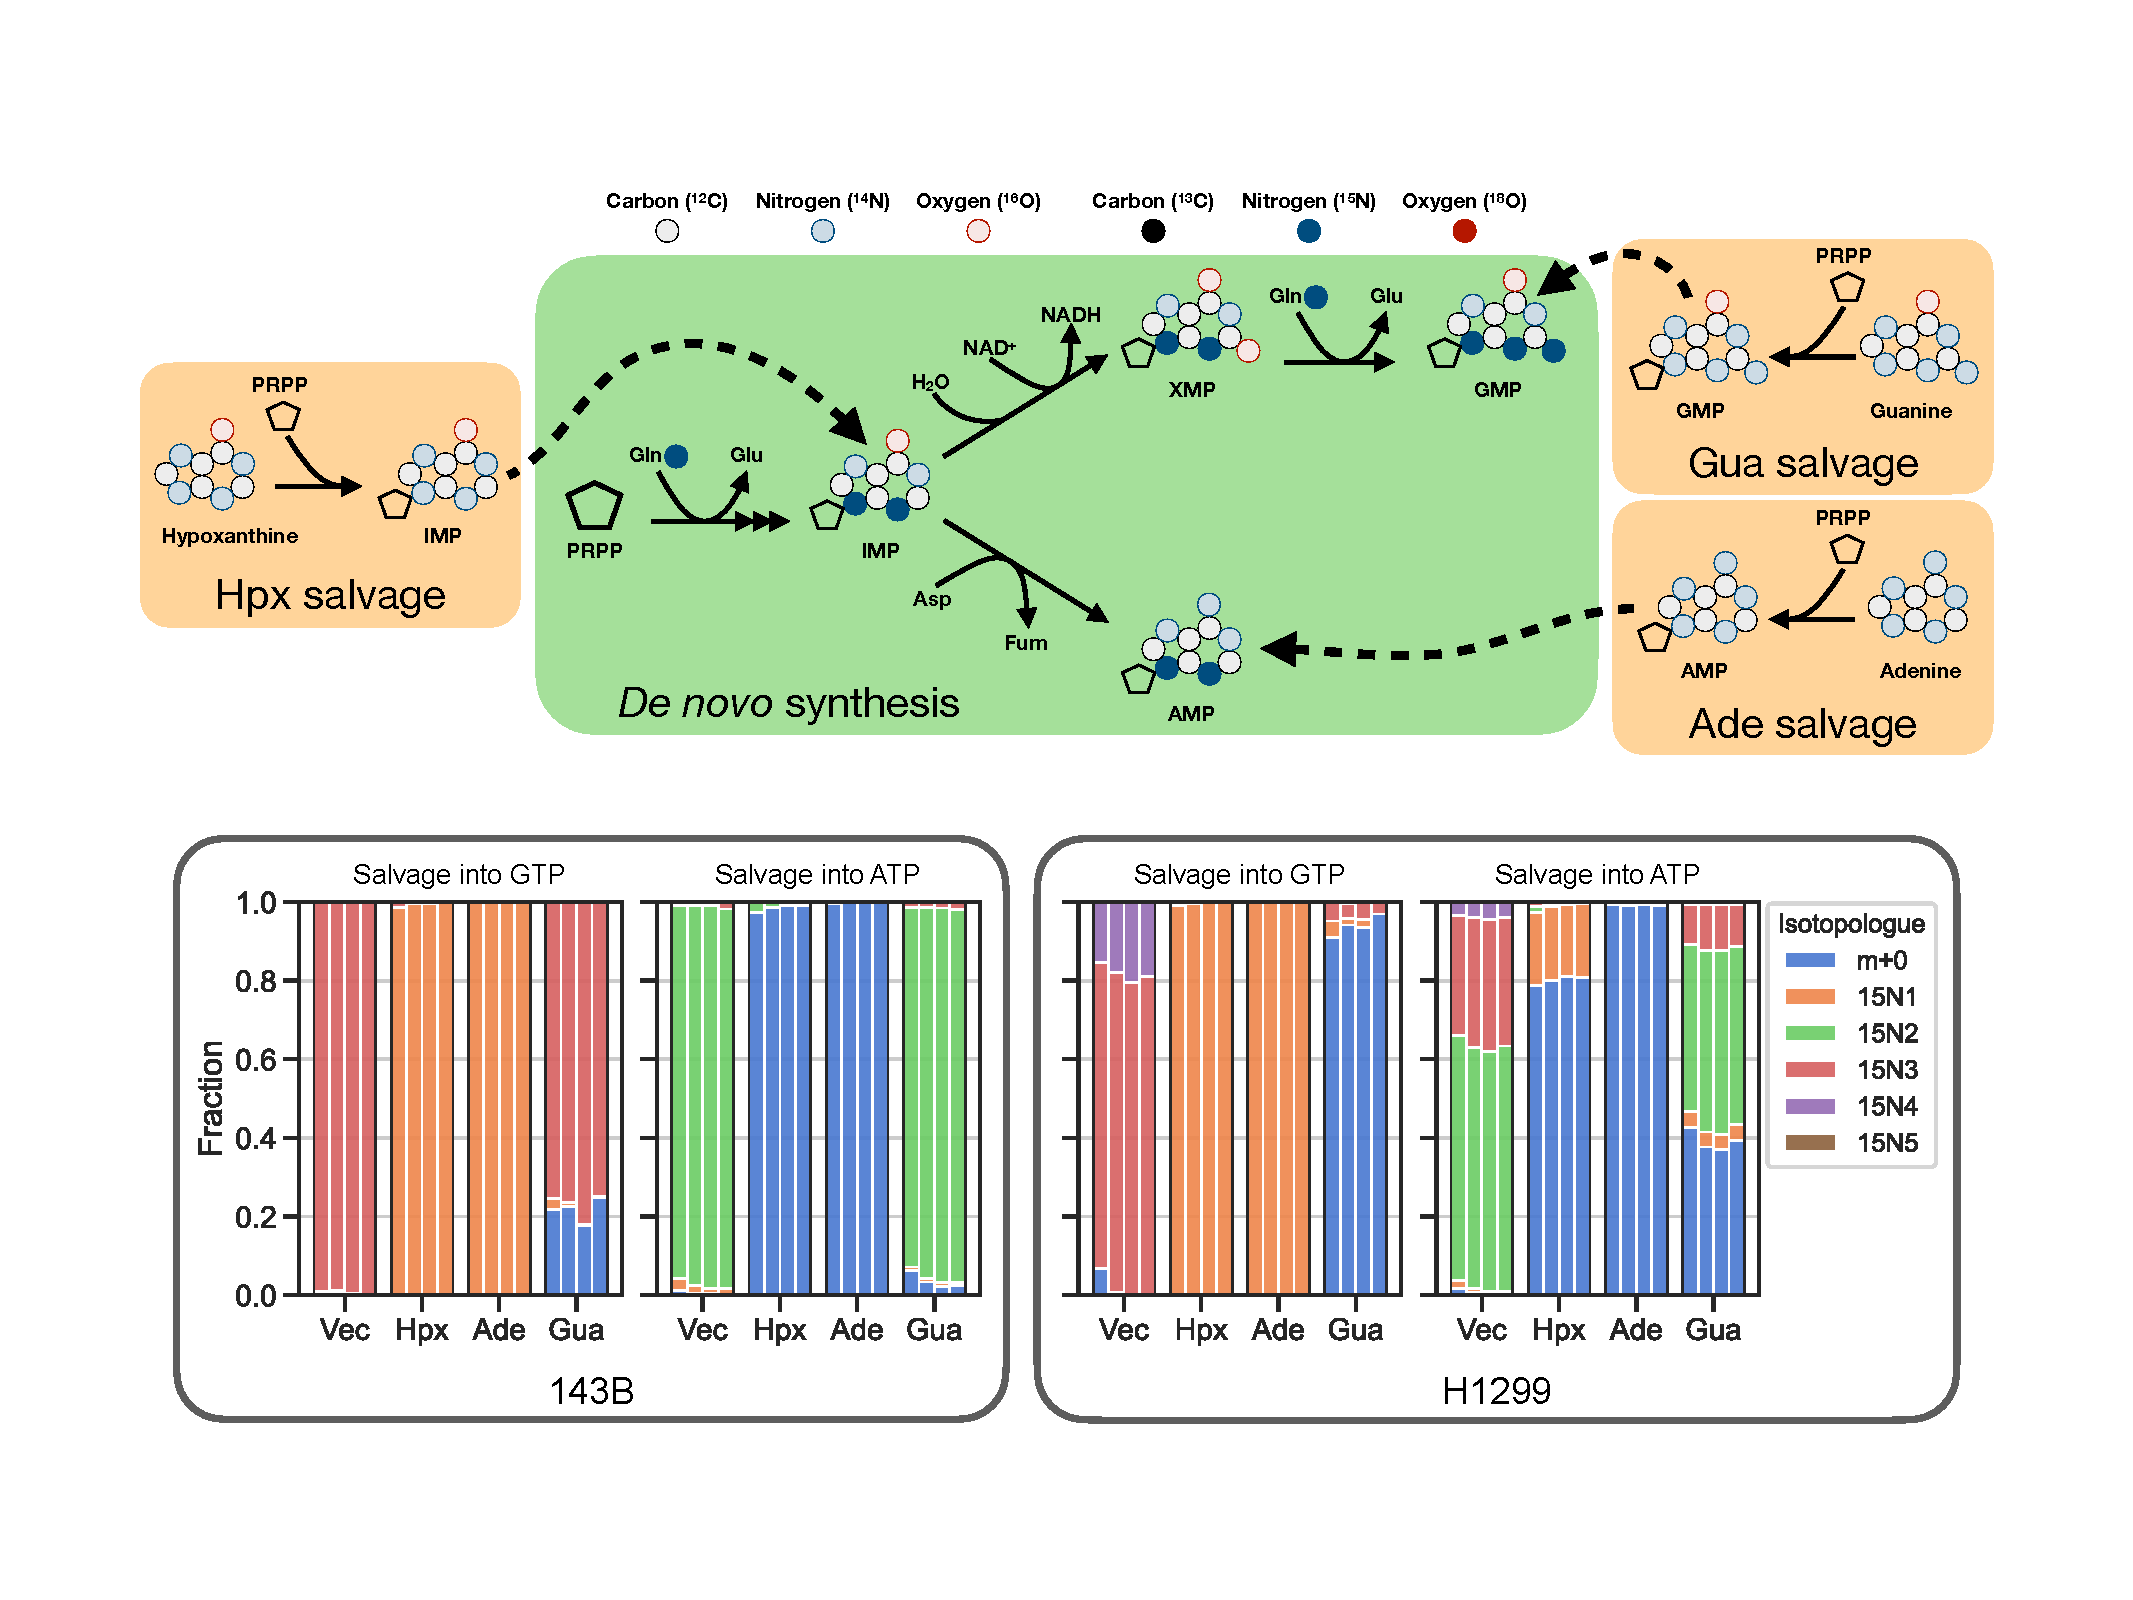
\includegraphics[width=0.98\textwidth]{figures/chap2/sal_frac_pur.pdf}
    \caption[Salvage into purines]{
    ggg
    }
    \label{fig:ch2:sal_frac_pur}
\end{figure}


\begin{figure}
    \centering
    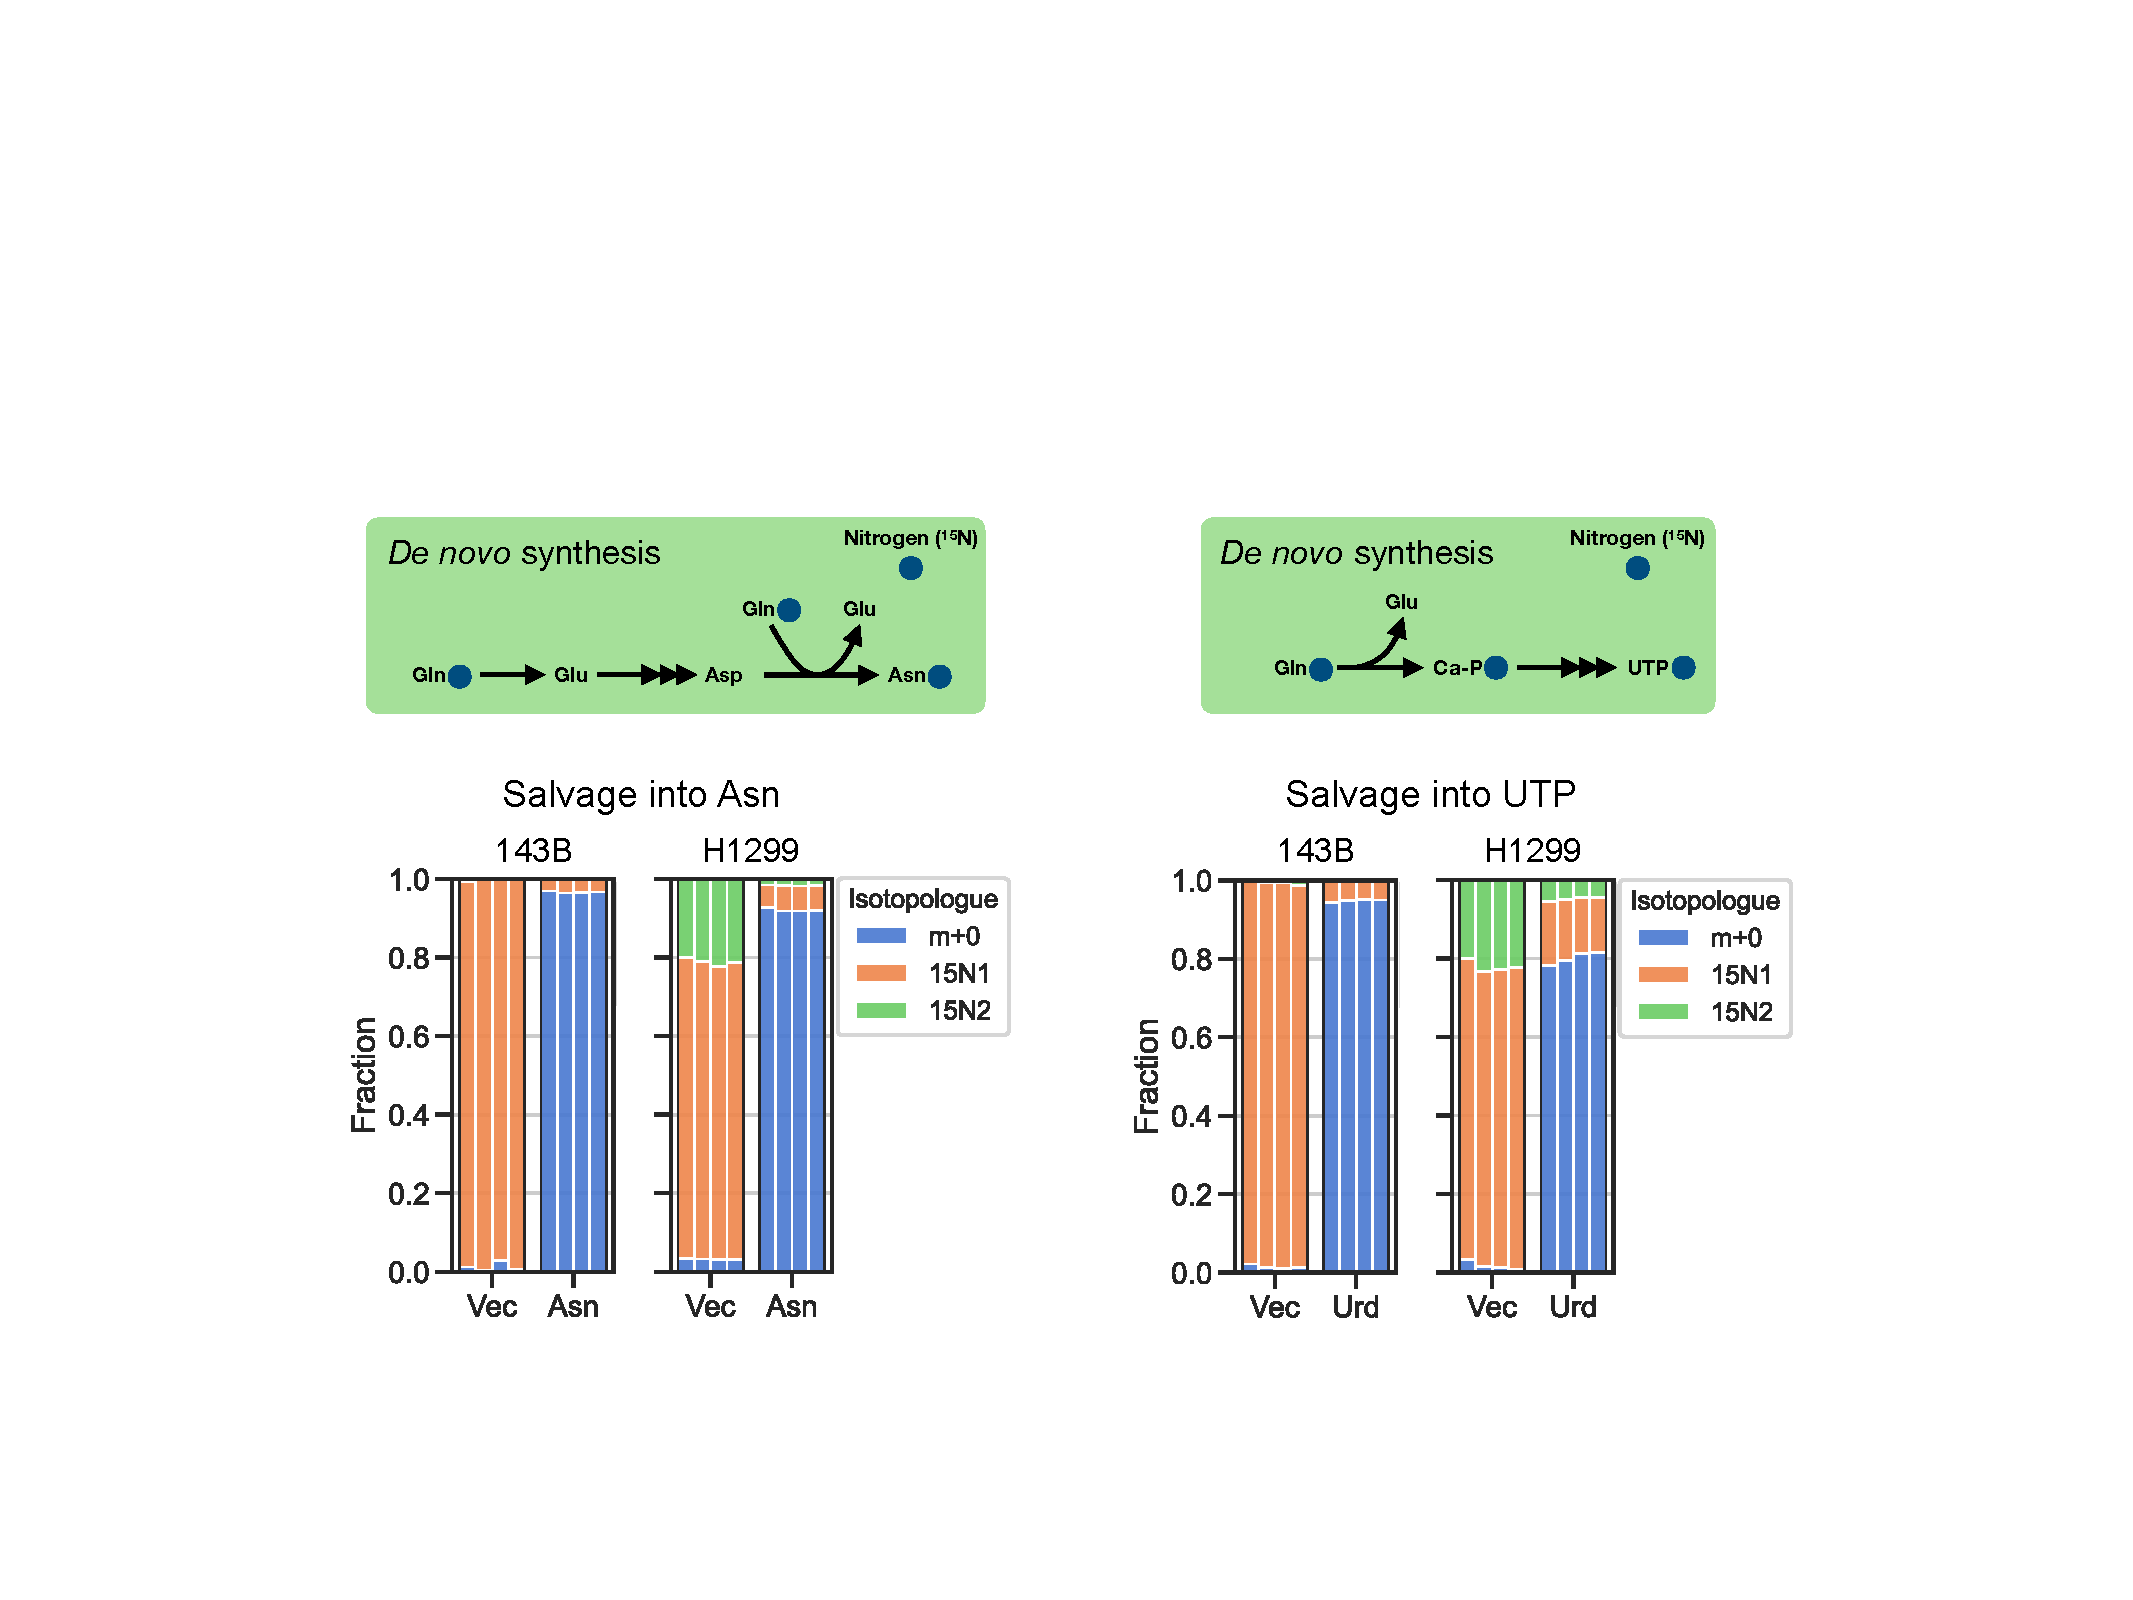
\includegraphics[width=0.8\textwidth]{figures/chap2/sal_frac_pyr-asn.pdf}
    \caption[Salvage into asparagine and pyrimidines]{
    ggg
    }
    \label{fig:ch2:sal_frac_pyr-asn}
\end{figure}









\begin{figure}
    \centering
    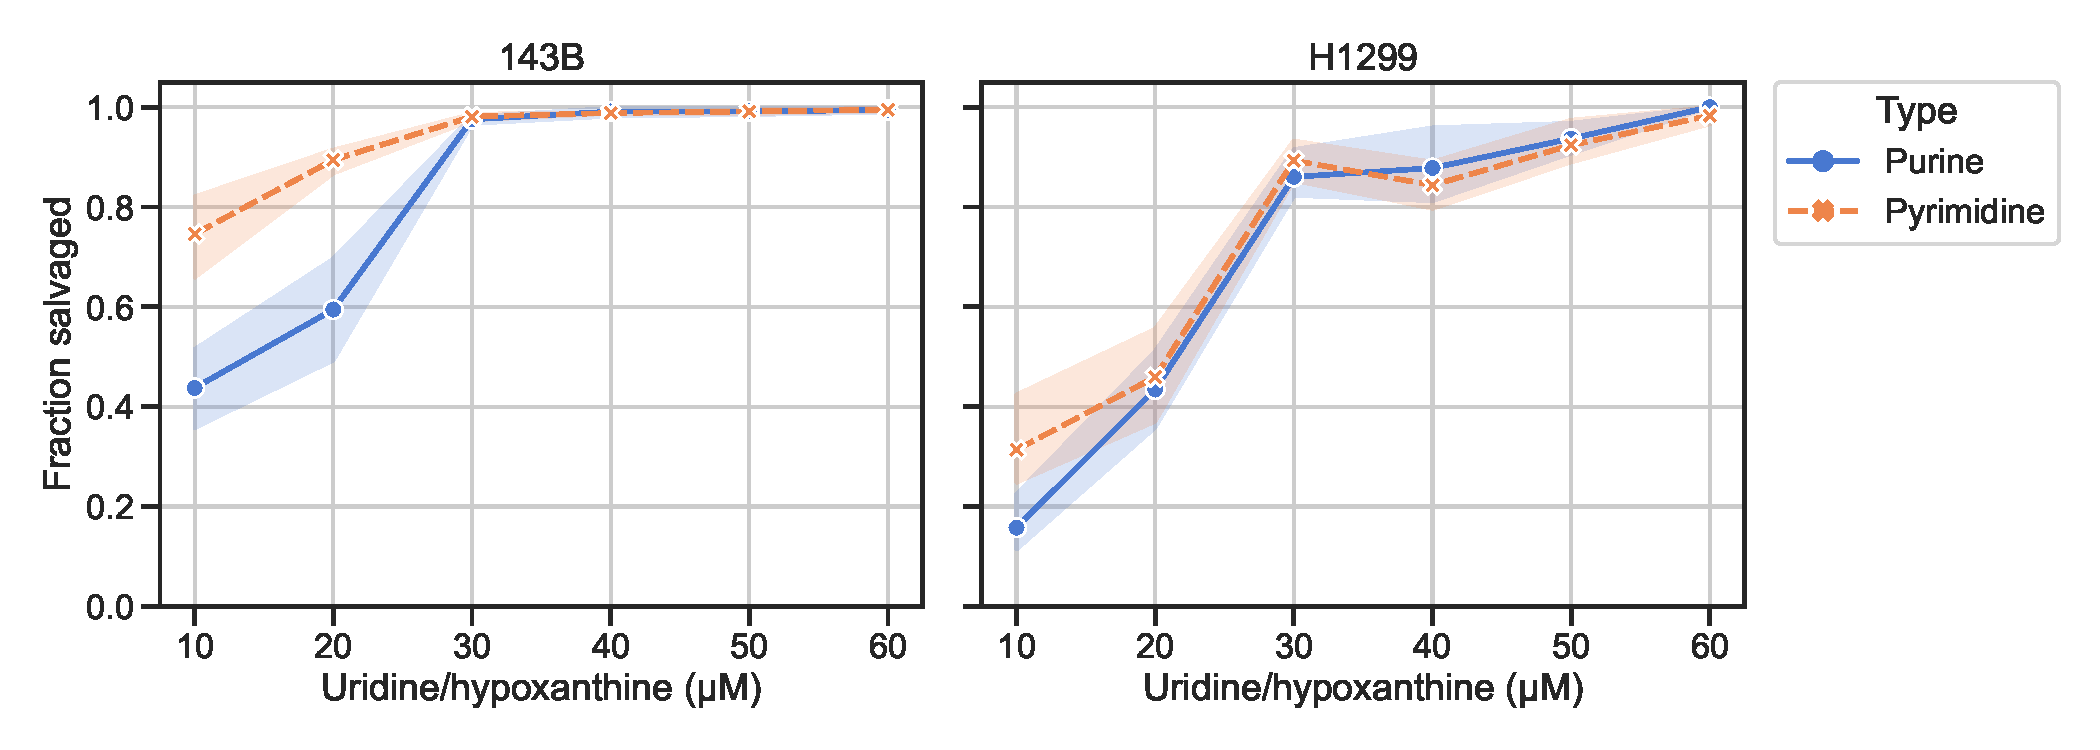
\includegraphics[width=0.95\textwidth]{figures/chap2/sal_frac_conc.pdf}
    \caption[Salvage as a function of Urd/Hpx concentration]{
    Fraction of purines (GDP, GMP, ADP and AMP) and pyrimidines (UDP, UMP, CDP and CMP) derived from salvage when cells are cultured in increasing concentrations of uridine/hypoxanthine.
    }
    \label{fig:ch2:sal_frac_conc}
\end{figure}












\section{Methods and Materials}

\subsection{Cell culture}
Cell lines were acquired from ATCC (143B, H1299, HT1080) and tested to be free from mycoplasma (MycoProbe, R\&D Systems).
Cells were maintained in Dulbecco’s Modified Eagle’s Medium (DMEM) (Gibco, 50-003-PB) supplemented with 3.7 g/L sodium bicarbonate (Sigma-Aldrich, S6297), 10\% fetal bovine serum (FBS) (Gibco, 26140079) and 1\% penicillin-streptomycin solution (Sigma-Aldrich, P4333).
Cells were incubated in a humidified incubator at 37°C with 5\% CO2.

\subsection{Proliferation assays}
Cells were trypsinized (Corning, 25,051 CI), resuspended in seeding media, counted (Beckman Coulter Counter Multisizer 4) and seeded overnight onto 6/12/24-well dishes (Corning, 3516;3513:3524) with an initial seeding density of 10,000 cells/mL and a volume of 4, 2 and 1 mL, respectively.
After overnight incubation, 3–6 wells were counted for a starting cell count at the time of treatment.
Treatment was initiated either by media switch or by spike-in of drug/metabolite from a 20-50x stock.
Experiments were conducted in (both for seeding and treatment) DMEM without pyruvate (Corning 50–013-PB) supplemented with 3.7 g/L sodium bicarbonate 10\% dialyzed fetal bovine serum (FBS) (Sigma-Aldrich, F0392) and 1\% penicillin-streptomycin solution, with or without sodium pyruvate (Pyr) (Sigma-Aldrich, P8574), 2-ketobutyric acid (AKB) (Sigma-Aldrich, K401), aspartate (Asp) (Sigma-Aldrich, A7219), asparagine (Sigma-Aldrich, A7094), uridine (Sigma-Aldrich, U3003), hypoxanthine (Cayman Chemical, 22254), adenine (Sigma-Aldrich, A2786) or guanine (Sigma-Aldrich, 51030) with concentration noted when relevant.
Drug treatments included rotenone (Sigma-Aldrich, R8875), metformin (Sigma-Aldrich, D150959), atpenin A5 (Cayman Chemical, 11898; AdipoGen, AG-CN2-0110; Abcam, ab144194; or Enzo Life Sciences, ALX-380–313), doxycycline hydrochloride (Sigma-Aldrich, D3447), antimycin A (Sigma-Aldrich, A8674), oligomycin A (Sigma-Aldrich, 495455) and DMSO vehicle (Sigma-Aldrich, D2650).
Cells were incubated in a humidified incubator at 37°C with 5\% CO2, then counted after 4–6 days.
Proliferation rate was reported as doublings per day and determined using the time and fold count difference between the starting and final counts and assuming a constant proliferation rate throughout the assay.




\subsection{Generation of nuclear RFP cell lines}
Nuclear RFP cell lines were generated using 1e5 transducing units of EF1A-nuclear RFP lentivirus (Cellomics Technology, PLV-10205-50) by spinfection.
Cells were seeded at 50\% confluency in 6 well dishes, lentivirus was added to fresh media with 8 µg/µL polybrene, then added to cells and followed by centrifugation (900g, 90 mins, 30°C).
Two days after infection, cells were sorted for high RFP expression using fluorescence-activated cell sorting (FACS).
High RFP cells were then expanded and single-cell cloned by limiting dilution, plating 0.5 cells/well on a 96 well plate.
Plates were then screened for RFP expression and localization using Incucyte S3 (Sartorius) and a suitable clone chosen, expanded, and used for all subsequent experiments.

\subsection{Lentiviral production and stable cell line generation}
jAspSnFR3 and jAspSnFR3-mRuby3 were first cloned into entry vector pENTR1A (Fisher, A10462) using NEBuilder HiFI DNA Assembly Cloning Kit (New England BioLabs, E2621).
These donor constructs were then used to transfer their insert into destination vectors: pLX304-CMV-Blast (Addgene, 25890), pLenti-CMV-Hygro (w117-1) (Addgene, 17454 a gift from Eric Campeau \& Paul Kaufman), or pLX304-CAG-Blast using LR Clonase II (Fisher, 11791100).
pLX304-CAG-Blast was generated in house by swapping the CMV promoter region of pLX304-CMV-Blast with a CAG promoter provided on synthetic DNA (Integrated DNA Technologies).
Each plasmid sequence was verified by whole plasmid sequencing (Plasmidsaurus).
Lentivirus was generated by co-transfection of HEK293T cells with destination vector plasmid DNA and the packaging plasmids pMDLg/pRRE (Addgene, 12251), pRSV-Rev, (Addgene, 12253) and pMD2.G (Addgene, 12259) using FuGENE transfection reagent (Fisher, PRE2693) in DMEM (Fisher, MT10017CV) without FBS or penicillin-streptomycin.
The supernatant containing lentiviral particles was filtered through a 0.45 µM membrane (Fisher, 9720514) and was supplemented with 8 µg/µL polybrene (Sigma, TR-1003-G) prior to infection.
For infection, cells were seeded at 50\% confluency in 6 well dishes and centrifuged with lentivirus (900g, 90 mins, 30°C).
After 24 hours the media was replaced with fresh media and after 48 hours cells were treated with either 1 µg/mL blasticidin (Fisher, R21001) or 150 µg/mL hygromycin (Sigma-Aldrich, H7772-1G) and maintained in selection media until all uninfected control cells died.
After selection, cells were expanded and single-cell cloned by limiting dilution, plating 0.5 cells/well using 2-3 96 well plates.
These clones were incubated until 10-30\% confluency and screened for high GFP and RFP signal using Incucyte S3 (Sartorius).
The highest expressing monoclonal cells were selected and further expanded on 6 well plates and again screened for fluorescence using the Incucyte.
From this a single clone was chosen, expanded and used for all subsequent experiments.
Different cell lines received different vector-sensor combinations: HEK293T cells were infected with pLX304-CAG-jAspSnFR3-mRuby3 (blasticidin), HT1080 with pLenti-jAspSnFR3-mRuby3 (hygromycin) and HT1080, H1299 and H1299 GOT1/2 DKO cells expressing nuclear RFP were infected with pLenti-jAspSnFR3 (hygromycin).

\subsection{Generation of GOT1/2 double knockout (DKO) cells}
Protocol and guide RNA generation was identical to that described in \cite{Hart2023-gp}.
Briefly, three chemically synthesized 2'-O-methyl 3’phosphorothioate-modified single guide RNA (sgRNA) sequences targeting GOT1 and GOT2 were purchased (Synthego; table \ref{tab:ch2:guides}).
A pool of all six sgRNAs for GOT1 and GOT2 were resuspended in nuclease-free water, combined with SF buffer (Lonza, V4XC-2032), and sNLS-spCas9 (Aldevron, 9212).
200,000 H1299 cells were resuspended in the resulting solution containing ribonucleoprotein complexes (RNPs) and electroporated using a 4D-Nucleofector (Amaxa, Lonza).
Nucleofected cells were then expanded and single-cell cloned by limiting dilution by plating 0.5 cells/well in a 96 well plate.
Gene knockout was confirmed using western blots.

\begin{table}[ht]
\caption{\label{tab:ch2:guides}CRISPR guides.}
\begin{tabular}{|l|l|}
\hline
Gene & sgRNA   sequence (5’-3’) \\
\hline
GOT1 & \begin{tabular}[c]{@{}l@{}}\texttt{CAGUCAUCCGUGCGAUAUGC}\\\texttt{GCACGGAUGACUGCCAUCCC}\\\texttt{CGAUCUUCUCCAUCUGGGAA}\end{tabular} \\
\hline
GOT2 & \begin{tabular}[c]{@{}l@{}}\texttt{UUUCUCAUUUCAGCUCCUGG}\\\texttt{CGGACGCUAGGCAGAACGUA}\\\texttt{UCCUUCCACUGUUCCGGACG}\end{tabular} \\
\hline
\end{tabular}
\end{table}


\subsection{Polar metabolite extraction}
For polar metabolite extraction, a plate was move to ice and the media was thoroughly aspirated.
Wells were washed thrice with cold saline (Fisher, 23293184), 1 mL 80\% HPLC grade methanol in HPLC grade water was added, cells were scraped with the back of a P1000 pipet tip and transferred to Eppendorf tubes.
Tubes were centrifuged (17,000g, 15 mins, 4°C) and a fraction of the supernatant containing polar metabolites was transferred to a new centrifuge tube and placed in a centrivap until dry.
The fraction of supernatant transferred was adjusted to correspond to that extracted from a 1 µL cell volume e.g. 50\% was transferred if the total cell volume extracted from was 2 µL.
The total cell volume extracted from was determined by counting cells on a parallel plate using a coulter counter.
Dried samples were reconstituted with 40 µL 80\% HPLC grade methanol, containing internal standards if appropriate, and transferred to vials for measurement by LCMS.

\subsection{Intracellular amino acid concentration measurements by isotope dilution}
Dried samples were reconstituted with 40 µL 80\% HPLC grade methanol containing 5 µM U-13C, U-15N labelled canonical amino acid mix (Cambridge Isotope Laboratories, MSK-CAA-1) and transferred to vials for measurement by LCMS.
The peak area for each amino acid was divided by its labelled standard to derive the response ratio.
The response ratio was then mapped to a calibration curve to infer the amino acid concentration and finally the intracellular concentration was calculated by correcting for each step introducing a dilution, including the use of the total cell volume.
To make the calibration curves a non-labelled amino acid mixture was made from an analytical amino acid standard without glutamine and asparagine (Sigma-Aldrich, A9906-1ML) and added glutamine (Sigma-Aldrich, 76523-100MG) and asparagine (Sigma-Aldrich, 51363-100MG) to match the concentration of the other amino acids.
Using this mix, three replicates of a 12 point 2-fold dilution series was made with a max concentration of 500 µM and a volume per dilution of 40 µL.
These were placed in a centrivap until dry and reconstituted with 40 µL 80\% HPLC grade methanol containing 5 µM U-13C, U-15N labelled canonical amino acid mix (Cambridge Isotope Laboratories, MSK-CAA-1) and transferred to vials for measurement by LCMS.
The peak area for each amino acid was divided by its labelled standard to derive the response ratio, then the best fitting calibration curves for each amino acid were chosen among either linear, power or a second-degree polynomial.
Each calibration curve was manually inspected for proper fit and measurements below or above the concentration range of the dilution series were discarded.

\subsection{Liquid Chromatography-Mass Spectrometry (LCMS)}
Metabolite quantitation was performed using a Q Exactive HF-X Hybrid Quadrupole-Orbitrap Mass Spectrometer equipped with an Ion Max API source and H-ESI II probe, coupled to a Vanquish Flex Binary UHPLC system (Thermo Scientific).
Mass calibrations were completed at a minimum of every 5 days in both the positive and negative polarity modes using LTQ Velos ESI Calibration Solution (Pierce).
Polar Samples were chromatographically separated by injecting a sample volume of 1 µL into a SeQuant ZIC-pHILIC Polymeric column (2.1 x 150 mm 5 mM, EMD Millipore).
The flow rate was set to 150 mL/min, autosampler temperature set to 10°C, and column temperature set to 30°C.
Mobile Phase A consisted of 20 mM ammonium carbonate and 0.1\% (v/v) ammonium hydroxide, and Mobile Phase B consisted of 100\% acetonitrile.
The sample was gradient eluted (\%B) from the column as follows: 0-20 min.: linear gradient from 85\% to 20\% B; 20-24 min.: hold at 20\% B; 24-24.5 min.: linear gradient from 20\% to 85\% B; 24.5 min.-end: hold at 85\% B until equilibrated with ten column volumes.
Mobile Phase was directed into the ion source with the following parameters: sheath gas = 45, auxiliary gas = 15, sweep gas = 2, spray voltage = 2.9 kV in the negative mode or 3.5 kV in the positive mode, capillary temperature = 300°C, RF level = 40\%, auxiliary gas heater temperature = 325°C.
Mass detection was conducted with a resolution of 240,000 in full scan mode, with an AGC target of 3,000,000 and maximum injection time of 250 msec.
Metabolites were detected over a mass range of 70-850 m/z.
Quantitation of all metabolites was performed using Tracefinder 4.1 (Thermo Scientific) referencing an in-house metabolite standards library using ≤5 ppm mass error.
For samples subjected to stable isotope tracing, peak areas were natural abundance corrected with IsoCor \cite{Millard2019-hv}, using experimentally determined tracer purity values.



\subsection{Nitrogen-15 tracing}

\subsubsection{Salvage fraction of individual components}
The fractional contribution of individual components into their respective aspartate consuming fates was determined in 143B and H1299 cells for the salvageable metabolites asparagine (Asn), uridine (Urd), hypoxanthine (Hpx), adenine (Ade) and guanine (Gua) along with a vehicle treatment (Vec).
The salvageable metabolites were spiked-in from a 20x stock solution to achieve a final concentration of: 500 µM Asn, 200 µM Urd, 100 µM Hpx, 100 µM Ade or 100 µM Gua.
The fraction of salvage was determined by stable isotope tracing, performed using both Gln amide\=/\textsuperscript{15}N (Cambridge Isotope Laboratories, NLM-557-PK) and Gln alpha\=/\textsuperscript{15}N (Cambridge Isotope Laboratories, NLM-1016-PK) in separate reactions and added to DMEM without glucose, glutamine, pyruvate and phenol red (Sigma, D5030) supplemented with 10\% dialyzed FBS, 1\% penicillin-streptomycin, 25 mM glucose (Sigma, G7528).
The combination of cell lines, salvageable metabolites and tracers gave 2x6x2=24 conditions which were labelled to steady-state by culturing for four passages with a 1/20 split at each passage.
At the end of the last passage each condition was split into four technical replicates and plated on 24 well dishes (Corning, 3524).
Upon reaching confluency, polar metabolites were extracted and submitted to LCMS with the above described technique.

\subsubsection{Salvage fraction as a function of concentration}
Seeded H1299 and 143B cells at 5,000 and 10,000 cells/well on a 6-well dish in DMEM containing Gln amide\=/\textsuperscript{15}N as described above.
Then added an equimolar mix of hypoxanthine and uridine from a 40x stock to a final concentration of 10, 20, 30, 40, 50, 60 µM in each of the 6 wells.
Fresh media was then added every four days and upon reaching confluency, polar metabolites were extracted and submitted to LCMS with the above described technique.








